\documentclass[10pt,a4paper]{article}
\usepackage{arabtex}
\usepackage[OT1,T1,LFE,LAE]{fontenc}
\usepackage[utf8]{inputenc}
\usepackage[arabic,english,farsi]{babel}
\usepackage{amsmath,amsfonts} % Math packages
\usepackage{amssymb}

\usepackage{multicol}

\usepackage{graphicx}
\usepackage{color}
\usepackage{float}
\usepackage{sidecap}
\usepackage{anysize}
\marginsize{2cm}{2cm}{2cm}{2cm}

\usepackage{listings}

\usepackage{appendix}

\usepackage[colorlinks=true,plainpages=true,citecolor=blue,linkcolor=blue,urlcolor=cyan]{hyperref}

%%% Equation and float numbering
\numberwithin{equation}{section}
\numberwithin{figure}{section}
\numberwithin{table}{section}


\newcommand{\horrule}[1]{\rule{\linewidth}{#1}}    % Horizontal rule

\newcommand{\titleText}{Static and Dynamic routing \\ Laboratory Manual}

\title{
\normalsize In the name of Allah\\
\vspace{10pt}
\LARGE\FR{بسم \allah\  الرحمن الرحیم}
\vspace{10pt}
\begin{center}
    %	\newcommand{\HRule}{\rule{\linewidth}{0.5mm}}
    \begin{minipage}{0.48\textwidth}
        \begin{flushleft}
            
\includegraphics[height=64pt,width=64pt]{../img/logo.png}
        \end{flushleft}
    \end{minipage}
    \begin{minipage}{0.48\textwidth}
        \begin{flushright}
            
\includegraphics[height=64pt]{../img/eng-logo.png}
        \end{flushright}
    \end{minipage}
\end{center}
\vspace*{-64pt}
%	\horrule{0.5pt} \\[0.4cm]
\huge \titleText\\
\vspace{40pt}
%	\horrule{2pt} \\[0.5cm]
}
\author{
	\huge University of Tehran\\
    \LARGE \FR{دانشگاه تهران}\\\\
    \LARGE School of Electrical and Computer Engineering\\
    \FR{دانشکده مهندسی برق و کامپیوتر}\\\\
    \Large Computer Network Lab\\
    \FR{آزمایشگاه شبکه‌های کامپیوتری}\\\\\\\\
    \normalfont
    Dr. Ahmad Khonsari - \FR{احمد خونساری}\\
    \href{mailto:a_khonsari@ut.ac.ir}{a\_khonsari@ut.ac.ir}\\\\
    \normalsize
    Amir Haji Ali Khamseh'i - \FR{امیر حاجی علی خمسه‌ء}\\
    \href{mailto:khamse@ut.ac.ir}{khamse@ut.ac.ir}\\\\
    \normalsize \href{mailto:m.borhani@ut.ac.ir}{Muhammad Borhani} - \FR{محمد برهانی}\\
	\normalsize \href{mailto:a.a.khordadi@ut.ac.ir}{Amirahmad Khordadi} - \FR{امیر احمد خردادی}\\
	\normalsize \href{mailto:sina\_kashipazha@ut.ac.ir}{Sina Kashi pazha} - \FR{سینا کاشی پزها}\\
	\normalsize \href{mailto:mashahsavand@ut.ac.ir}{Mohammad Ali Shahsavand} - \FR{محمد علی شاهسوند}
}

\date{\vspace{30pt}\today\\\vspace{10pt}{\selectlanguage{farsi}\today}}

\usepackage{fancyhdr}
\pagestyle{fancy}
%\pagestyle{fancyplain}
\fancyhf{}
\fancyhead[L]{\footnotesize Computer Network Lab \\ \FR{آزمایشگاه شبکه‌های کامپیوتری}}
\fancyhead[R]{\footnotesize \titleText}
\fancyfoot[R]{\footnotesize School of Electrical and Computer Engineering\\\FR{دانشکده مهندسی برق و کامپیوتر}}
\fancyfoot[C]{\thepage}
\fancyfoot[L]{\footnotesize University of Tehran \\ \FR{دانشگاه تهران}}
\renewcommand{\footrulewidth}{0.8pt}
\renewcommand{\headrulewidth}{1pt}            % Remove header underlines
\renewcommand{\footrulewidth}{1pt}                % Remove footer underlines
\setlength{\headheight}{13.6pt}


\begin{document}
    \selectlanguage{english}

    %\vspace*{-1.5cm}
    \maketitle


    \pagebreak

    \section*{A Simple Router Experiment}
    As in the previous lab, we will divide the students into four groups, each with two workstations, a router, and two hubs, which are to be connected as shown in Figure 4.10.
    The IP addresses of the routers and hosts are given in Table 4.2 and Table 4.3, respectively.
    \begin{figure}[H]
        \centering
        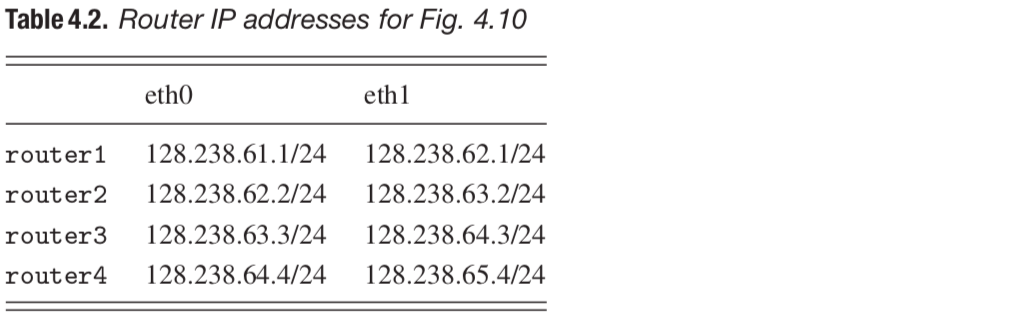
\includegraphics[width=0.9\textwidth]{img/table4-2.png}
    \end{figure}
    \begin{figure}[H]
        \centering
        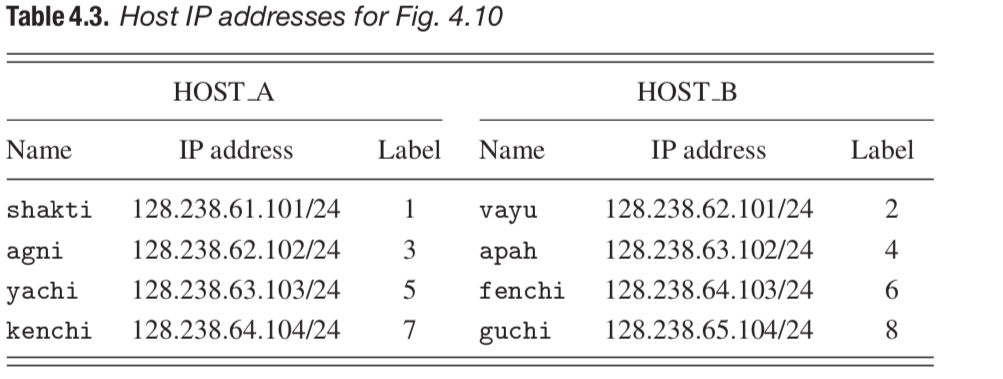
\includegraphics[width=0.9\textwidth]{img/table4-3.png}
    \end{figure}
    \begin{figure}[H]
        \centering
        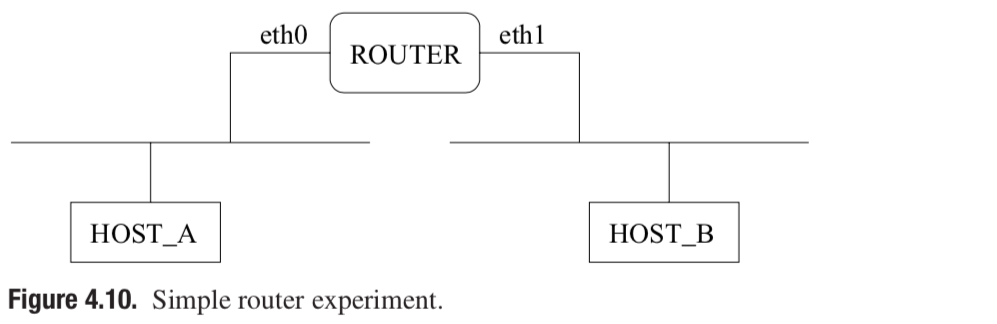
\includegraphics[width=0.9\textwidth]{img/figure4-10.png}
    \end{figure}

    \section{Exercise 1}
    Configure the IP addresses of your workstations and the router as shown in Figure 4.10, Table 4.2 and Table 4.3. \\
    Initially your host’s routing table has no entry for the subnet on the other side of the router.
    In order to be connected, you need to add a routing entry for the other subnet in the routing table of your workstation (see section 4.3.1). \\
    Run \textbf{tcpdump -en} on your machine, and \textbf{tcpdump -en} on your partner’s machine in the other subnet simultaneously: \\
    \textbf{tcpdump -en host} \textit{remote-host} and \textit{your-machine} \\
    Send \textbf{ping} messages continuously to your partner’s machine: \\
    \textbf{ping -sv} \textit{remote-host} \\
    After receiving the tenth echo reply, quit \textbf{ping} and save the \textbf{tcpdump} outputs from both machines.
    Also, copy the \textbf{ping} output. \\
    During this exercise, don’t run the \textbf{ping} program at the same time.
    For clean results, do your experiments in turn.
    \subsubsection*{Lab Report}
    \begin{itemize}
        \setlength{\itemindent}{0pt}
        \item When a packet was sent to a workstation in the other subnet, explain how the source and destination Ethernet addresses were changed.
        \item What are the source and destination addresses in the IP and Ethernet headers of a packet that went from your machine to the router?
        \item What are the source and destination addresses in the IP and Ethernet headers of a packet that went from the router to your partner’s machine?
        \item Answer the above two questions, but now for the echo reply that was returned from your partner’s machine.
    \end{itemize}
    \subsubsection*{ Lab Report}
    \begin{itemize}
        \setlength{\itemindent}{0pt}
        \item Use the \textbf{tcpdump} outputs from both machines to calculate the average delay that a packet experienced in the router. Note that the system times of the two machines might be different. Show all the steps and submit the \textbf{tcpdump} outputs with your report.
        \item Compare this value with the previous value in the case of the bridge. Which, a router or a bridge, is faster? Why?
    \end{itemize}



    \section*{RIP exercises}
    In this section, we will examine the operation of RIP. To enable the RIP routing process in a router, use the following commands in the \textit{Global Configuration} mode. \\
    \texttt{Router(config)\#} \textbf{router rip} \\
    \texttt{Router(config)\#} \textbf{network} \textit{network-number}, \\
    where \textit{network-number} could be 128.238.0.0. To remove the network, use: \\
    \texttt{Router(config)\#} \textbf{no network} \textit{network-number}, \\
    To shutdown the RIP process, use: \\
    \texttt{Router(config)\#} \textbf{no router rip} \\
    Consider Figure 4.11 as our network topology for this section.
    Since the IP address of ethernet1 in router4 is the only interface which is different from the initial configuration in Appendix B, we will reboot all the four routers to restore their default configurations, and change the IP address on the ethernet1 in router4 only. Since our workstations started \textbf{routed} at boot-up time, no further action is needed to run RIP on the workstations. \footnote{The lab instructor should make sure that the IP-Forwarding function is enabled in each host.}
    \begin{figure}[H]
        \centering
        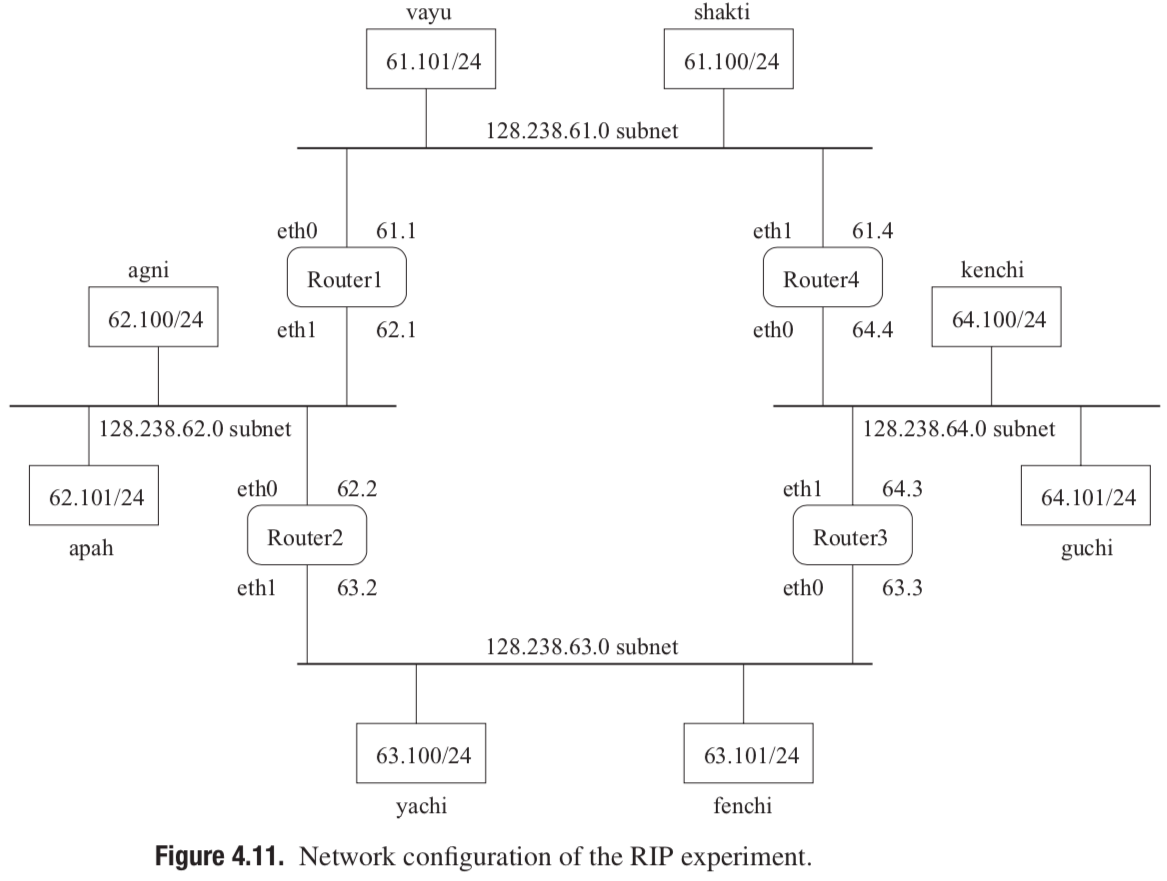
\includegraphics[width=0.9\textwidth]{img/figure4-11.png}
    \end{figure}
    \section{Exercise 2}
    Connect the routers and hosts and change the IP addresses of the workstations and router4 as shown in Figure 4.11.
    Also, make sure that your workstation has no other routing entries than your own subnet and your loopback interface.
    For how to remove an entry from the host routing table, see Section 4.3. \\
    Run the RIP process in each router.
    To avoid confusion, each router should be configured by only one person. \\
    After starting RIP in all the routers, test connections to other hosts by pinging them.
    Once you can successfully reach all the hosts, run the following command to capture the RIP messages sent on your subnet: \\
    \textbf{tcpdump -x -s 100 -c 4 -w exe2.out udp port 520} \\
    Save the routing table in your workstation.
    Note the number of hops needed to reach destinations other than in your own subnet. \\
    Run \textbf{wireshark exe2.out \&} to load the packet trace recorded by the above \textbf{tcpdump} command.
    Mark and print two different RIP messages captured in your subnet (see Exercise 6 of Chapter 1).
    Exchange the printed RIP messages with students in other groups.
    You need eight different RIP messages for your lab report.
    \subsubsection*{Lab Report}
    \begin{itemize}
        \setlength{\itemindent}{0pt}
        \item Explain why you can only get two different RIP messages in your subnet.
        Was a RIP packet forwarded by the routers?
        Why?
        \item Draw the format of one of the saved RIP response packets from your sub- net, including the IP and UDP headers and the RIP message (see Figs 0.13, 0.14, and 4.4). Identify each field, and express their values in decimal format.
        \item For the other seven RIP response packets collected, explain the contents of the RIP messages only, excluding IP and UDP headers.
    \end{itemize}
    \begin{itemize}
        \setlength{\itemindent}{0pt}
        \item Draw the distance tables and the routing tables in the routers based on Figure 4.11, assuming that number of hops is used as the metric.
        \item Verify the routing tables using the RIP messages you captured.
    \end{itemize}



    \section{Exercise 3}
    In this exercise we will examine how RIP responds to link failures.
    Send \textbf{ping} message continuously from \texttt{apah} to \texttt{yachi} and start \textbf{tcpdump} on \texttt{apah}.
    Let the two programs run during this exercise. \\
    Disconnect the cable from the \texttt{ethernet0} port of \texttt{router2} from the hub in the 128.238.62.0 subnet, and type the \textbf{time} command to get the current time. \\
    Observe the \textbf{ping} and \textbf{tcpdump} windows.
    When the connection is re-established, type the \textbf{time}  command again.
    See how much time RIP takes to alter the routing table in your workstation to the new topology. \\
    Once you can successfully reach other hosts, connect the cable to the original position.
    Again, measure the time that RIP takes to change your routing table.
    \subsubsection*{Lab Report}
    \begin{itemize}
        \setlength{\itemindent}{0pt}
        \item Compare this time with the previous value in the spanning tree experiment.
        \item Explain why it takes this time for RIP to react to the route change.
        Refer to Section 4.2.4 for RIP operation and default timer values.
    \end{itemize}


    \section*{Routing experiments with ICMP}
    \section{Exercise 4}
    Eliminate the routing entries for subnets other than your own and the loopback interface.
    Save the routing table for your lab report. \\
    Create a default routing entry using one of the routers directly connected to your workstation. \\
    While \textbf{tcpdump -enx -s 100 ip proto 1} is running, send \textbf{ping} messages to a host that is three hops away through the default router. \\
    After capturing an ICMP redirect message, save the \textbf{tcpdump} output, the \textbf{ping} output, and your workstation’s routing table.
    You may need to \textbf{ping} the same host several times in order to get your routing table updated.
    \subsubsection*{Lab Report}
    \begin{itemize}
        \setlength{\itemindent}{0pt}
        \item Submit what you saved in Exercise 4.
        \item Identify every field in the ICMP redirect message (see Figure 4.2).
        \item Compare the original routing table with the new routing table. Explain the meaning of the flags of the new entry.
    \end{itemize}


    \section*{OSPF exercise}
    In order to enable OSPF in the routers, you need to create an OSPF routing process first.
    Then, define the range of IP addresses to be associated with the routing process and assign area IDs for these IP addresses, using the following commands: \\
    \texttt{Router(config)\#} \textbf{router ospf} \textit{process-id}, \\
    \texttt{Router(config)\#} \textbf{network} \textit{address wildcard-mask} \textbf{area} \textit{area-id} \\
    \textit{Process-id} is a numeric value local to the router.
    It does not have to match \textit{process-id}s on other routers.
    \textit{address} is the network address of the interface on which the OSPF process runs (128.238.0.0 in our case).
    \textit{wildcard-mask} helps reduce the number of configuration commands.
    0 is a match and 1 is a “don’t care” bit (0.0.255.255 in our case).
    \textit{area-id} is the number of the area that the interfaces belong to (see Figure 4.7).
    It can be any integer between 0 and $2^{32} - 1$ or can have an IP address form.
    Note that 0 is reserved for the backbone. \\
    The above commands are required to configure OSPF, while other tasks (configuring interface parameters, configuring area parameters, etc.) are optional.
    For more information on other configuration tasks, refer to the router manual. \\
    Consider Figure 4.13 for our OSPF experiment.
    The lab instructor should reboot the routers to restore their default configurations.
    \begin{figure}[H]
        \centering
        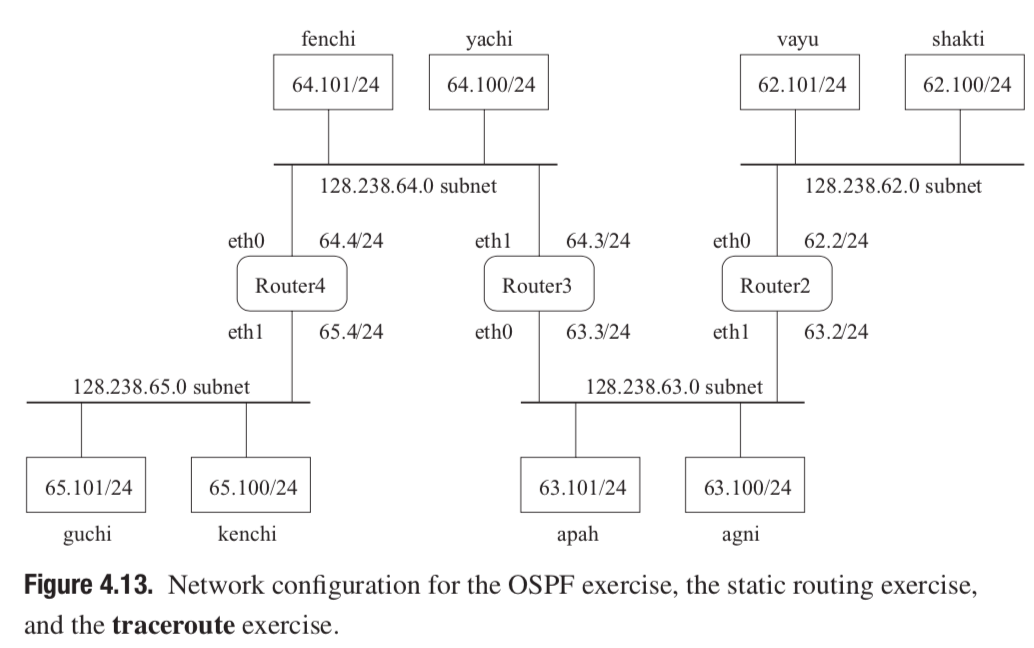
\includegraphics[width=0.9\textwidth]{img/figure4-13.png}
    \end{figure}

    \section{Exercise 5}
    After connecting the cables properly, change the host IP addresses as given in Figure 4.13 You need to remove the default route added in Exercise 4 from the host routing table.
    Note that the router interfaces are set as Fig. 4.13 by default. \\
    Run the following command to capture any OSPF packets: \\
    \textbf{tcpdump -x -s 120 ip proto 89} \\
    Login to a directly connected router and start the OSPF process.
    Set the argument \textit{area-id} to 1 for all the routers. \\
    The workstations in our lab run \textbf{routed} (which uses RIP).
    The routing daemon supporting OSPF, \textbf{gated}, is not installed.
    In order to reach the routers and hosts in the other subnets, you need to add a default router in your host’s routing table. \\
    Examine the routing table in each router (see Section 4.3).
    When the routing table gets an entry for the network that is not directly connected, kill the \textbf{tcpdump} process and save the \textbf{tcpdump} output. \\
    Collect the \textbf{tcpdump} outputs from other subnets.
    Study the various types of OSPF packets from the \textbf{tcpdump} outputs. \\
    You can display OSPF information in a router using the following commands in the \textit{Privileged EXEC} mode.
    \begin{verbatim}
        show ip ospf
        show ip ospf database [router|network|summary|asb-summary|external|database-summary]
        show ip ospf interface ethernet [0|1]
        show ip ospf neighbor
        show ip ospf virtual-links
    \end{verbatim}
    \subsubsection*{Lab Report}
    \begin{itemize}
        \setlength{\itemindent}{0pt}
        \item Draw the common header of a saved OSPF message, giving the decimal values of the header fields (see Fig. 4.8).
        \item Submit the routing tables you collected from the routers.
    \end{itemize}

    \section*{Static routing experiment}
    In this experiment, we reuse the network as shown in Figure 4.13.

    \section{Exercise 6}
    After checking the wiring, as shown in Figure 4.13, reboot the routers to restore their initial settings.
    Check the IP addresses of the workstations as shown in Figure 4.13. \\
    Remove all the routing entries other than your own subnet and the loopback interface from your host routing table.
    Save the output of \textbf{netstat -rn} before building your workstation’s routing table. \\
    Examine Figure 4.13 and build your host’s static routing table manually. \\
    \textbf{Telnet} to a router that is directly connected to your workstation, and save its routing table before building any route.
    Save the routing table of the other router if you have one more router connected directly.
    You may not be able to \textbf{telnet} to a router that is not directly connected.
    In this case, copy the initial routing table of these routers from students in other subnets later. \\
    Now configure the routing table in each router.
    See Section 4.3 for commands and syntax on manipulating router routing tables.
    Note that each router should be configured by one person only. \\
    Use \textbf{ping} to test the connections.
    When you can reach all other subnets successfully,\footnote{Even when the routing table in your workstation and all the routers are configured perfectly, you may not be able to \textbf{ping} a remote host, if the routing table in the remote host is incorrect.
    When you can get \textbf{ping} reply messages from all the interfaces of the routers successfully, your work is done for this exercise.} save the routing tables in your workstation and all the routers for the lab report.
    \subsubsection*{Lab Report}
    Submit the routing tables saved in this exercise.


    \section*{Traceroute experiment}
    In this exercise, we use the same network and configuration of the previous exercises, and use \textbf{traceroute} to find a multi-hop path.

    \section{Exercise 7}
    Execute \textbf{tcpdump -enx -s 100 host} \textit{your-host} \textbf{and} \textit{remote-host} on your host, where \textit{remote-host} is a workstation at least two hops away. \\
    Then, execute \textbf{traceroute} \textit{remote-host} to find the route from your host to the remote host. \\
    Save the output of both \textbf{traceroute} and \textbf{tcpdump}.

    \subsubsection*{Lab Report}
    Submit what you saved in this exercise. \\
    From the \textbf{tcpdump} output, explain how the multi-hop route was found.
    Explain the sequence of the ICMP messages used.
\end{document}